\documentclass[a4paper]{report}
\usepackage[spanish]{babel}
\selectlanguage{spanish}
\usepackage[utf8]{inputenc}
\usepackage[T1]{fontenc}
\usepackage{pdfpages}
\usepackage[a4paper,top=2cm,bottom=2cm,left=2cm,right=2cm]{geometry}
\usepackage{amsmath, amsthm, amsfonts}
\usepackage{graphicx}
\usepackage{minitoc}
\usepackage{color}
\usepackage{listings}
\usepackage{hyperref}
\usepackage{multicol}
\usepackage{float}
\usepackage{array}
\usepackage[none]{hyphenat}
\usepackage{appendix}
\usepackage[pdf]{graphviz}

\graphicspath{ {images/} }

\hypersetup{
    colorlinks=true, % make the links colored
    linkcolor=black, % color TOC links in blue
    urlcolor=red, % color URLs in red
    linktoc=all % 'all' will create links for everything in the TOC
}

\lstset{
basicstyle=\ttfamily,
captionpos=b,
frame=single,
texcl=true
}

\def\blankpage{%
      \clearpage%
      \thispagestyle{empty}%
      \addtocounter{page}{0}%
      \null%
      \clearpage}
    
\title{Desarrollo de la Lógica Proposicional y de Primer Orden bajo el paradigma funcional y la orientación Web.}
\author{Víctor Ramos González\\\\
   Tutor: Fernando Sancho Caparrini\\
   \textit{Ciencias de la Computación e Inteligencia Artificial}\\
   E.T.S. Ingeniería Informática\\
   Universidad de Sevilla\\
  \vspace{8cm}
  \date{Curso 2019/20}
}

\newcolumntype{P}[1]{>{\centering\arraybackslash}p{#1}}



\setlength{\parskip}{1em} 
 
\sloppy
\begin{document}

\renewcommand{\tablename}{Tabla}
\renewcommand{\appendixname}{Anexo}
\renewcommand{\appendixtocname}{Anexos}
\renewcommand{\appendixpagename}{Anexos}

\newcommand{\toDo}{\fbox{TO DO}}
\dominitoc

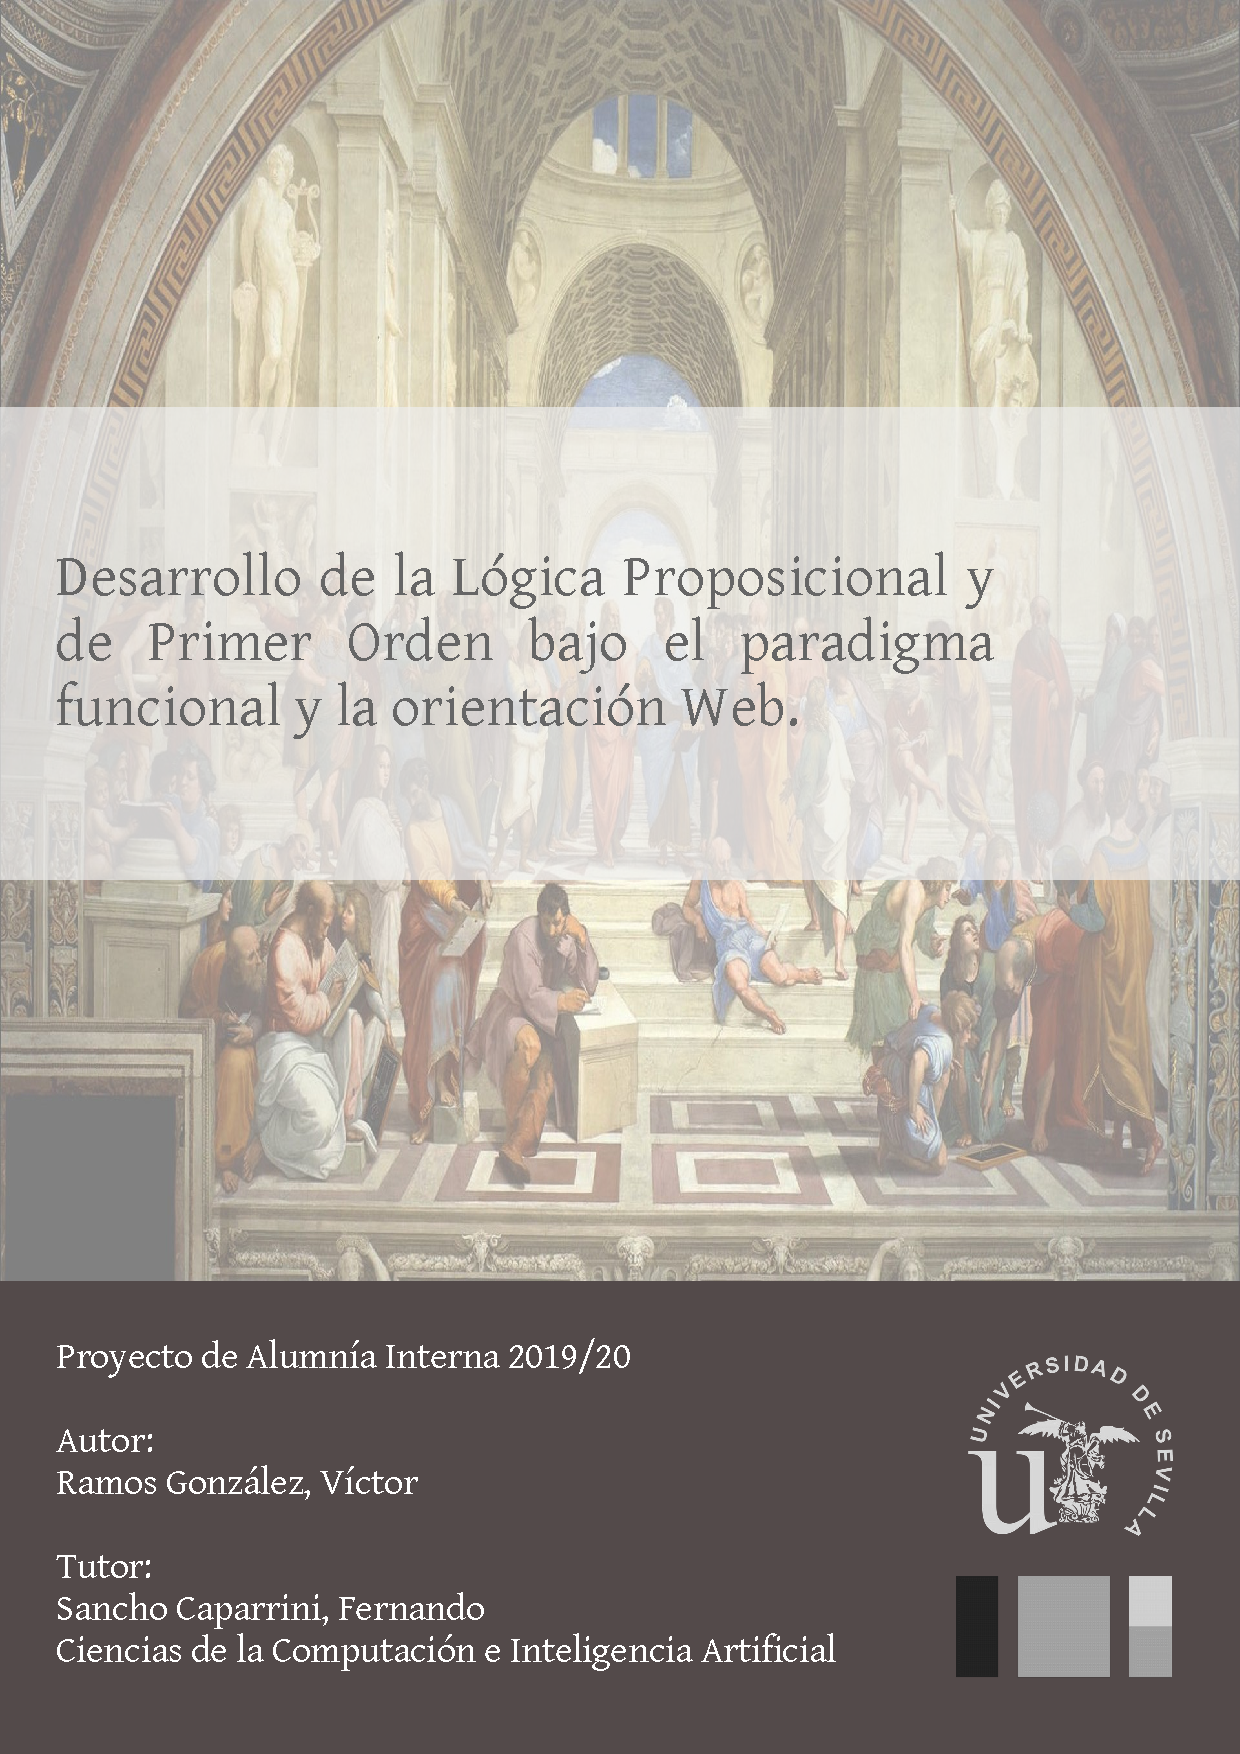
\includepdf[pages={1}]{archivos/titlepage.pdf}


\blankpage

\maketitle


\begin{abstract}

El proyecto aborda los conceptos y algoritmos básicos de la Lógica Proposicional y la Lógica de primer, desde un punto de vista implementativo a través de un lenguaje encuadrado en el paradigma funcional (Elm).

El proyecto, basado en la asignatura de Lógica Informática, busca una doble finalidad, por un lado servir como una somera introducción a la programación declarativa al mismo que tiempo que proporcionar al alumnado  herramientas intuitivas y de sencillo uso en la realización de los ejercicios que apoyen los contenidos teóricos que se desarrollan en dicha asignatura.
\end{abstract}

\tableofcontents

\newpage


\chapter{Introducción. Objetivos y organización del proyecto}
\renewcommand{\mtctitle}{}
\mtcskip
\minitoc
\newpage

\section{Introducción}

El proyecto surge desde 2 inspiraciones: por un lado mi interés para con el desarrollo de la Teoría de la Lógica Matemática y por otro mi gusto y vocación en el ámbito docente, por lo que la idea de poder desarrollar una herramienta, enfocada al ámbito académico, para el trabajo con diversas lógicas, me despertó una gran motivación.

El presente proyecto, pretende llevar a cabo el  desarrollo de una herramienta que permita dar un punto de vista más práctico de los contenidos de la Lógica Proposicional y la Lógica de Primer Orden, al mismo tiempo que sirva al alumno como complemento para la comprensión de los conceptos y la realización y razonamiento de los ejercicios relacionados con dichos conceptos.

El desarrollo del proyecto se llevará a cabo bajo el paradigma de la programación funcional (con el lenguaje Elm) y la posibilidad que este ofrece para su sencilla implementación web para permitir la elaboración de una herramienta interactiva, sencilla y accesible.

\section{Antecedentes del proyecto}

Tras haber cursado la asignatura de Lógica Informática con el profesor D. Fernando Sancho Caparrini, director de este proyecto, se despertó mi gusto por la Teoría de la Lógica Matemática y Computacional y tras comprobar que son excasas las herramientas prácticas que abordan estos contenidos desde un punto de vista académica se planteó la realización de un proyecto análogo con el uso de otras herramientas y otros lenguajes, aunque finalmente, el proyecto no pudo llevarse a cabo.

No obstante la idea del desarrollo de esta herramienta seguía en mente y tras cursar la asignatura de \textit{Programación Declarativa} con el profesor D. Miguel Ángel Martínez del Amor y el lenguaje Haskell, planteé a Fernando la posibilidad de retomar el proyecto pero bajo el lenguaje \textit{Haskell} y el paradigma funcional. Sin embargo, una herramienta similar había sido desarrollada por el profesor D. José Antonio Alonso Jiménez en su obra \textit{Lógica en Haskell}, en la que realiza un amplio desarrollo de la Lógica Proposicional y completada por D. Eduardo Paluzo en su TFG, en el que aborda con una metodología análoga al anterior los conceptos de la Lógica de Primer Orden. 

Fue entonces cuando Fernando me propuso realizar una `traducción' (incorporando algunos aspectos complementarios) de dichas obras, dentro del mismo paradigma pero bajo otro lenguaje, orientado además al ámbito Web, el lenguaje \textit{Elm}.

\section{Objetivos del proyecto}
Como hemos comentado anteriormente, el proyecto persigue un objetivo dual:

\begin{itemize}
\item Por un lado, desarrollar una librería completa (compuesta de una serie de módulos) en el lenguaje \textit{Elm}, que nos permita llevar a cabo la definición de conjuntos de fórmulas proposicionales y de primer orden, y la aplicación de los algoritmos básicos para tratar de abordar la satisfactibilidad de los mismos, mediante la aplicación de algoritmos fundamentales.

\item Por otro lado, llevar a cabo una implementación Web, de manera que el sistema sea usable por los alumnos de manera sencilla y visual, para que sirva como complemento de los conceptos y técnicas abordados en la asignatura de \textit{Lógica Informática.}
\end{itemize}

Además podemos destacar una serie de objetivos u competencias complementarias que aporta la realización de este proyecto como es la introducción al manejo de herramientas de publicación y manejo de versiones (\textit{git}) o el manejo de \textit{Latex}.


\section{Estructura del proyecto}

El proyecto se estructará en 2 partes fundamentales:

\subsection{Módulos funcionales}

En primer lugar, se llevará a cabo desarrollo de una librería completa que nos permita trabajar, tanto con fórmulas del ámbito de la Lógica Proposicional como de la Lógica de Primer Orden mediante la implementación de distintos módulos funcionales, que se describen detalladamente a lo largo de este documento y que recogen las estructuras, algoritmos y funciones necesarias para abordar los conceptos y técnicas vistas en la asignatura de \textit{Lógica Informática}.

\subsection{Interfaz gráfica (GUI)}

En segundo lugar, se llevará a cabo el diseño e implementación de una interfaz web, que permita el uso del sistema desde 2 ámbitos distintos, por una parte desde el punto de vista de la definición de fórmulas y la aplicación directa de las funciones y técnicas sobre dichas fórmulas, y en segundo lugar la posibilidad de trabajar con las funciones de una manera más cercana a la \textit{Programación Declarativa}.

Para ello se combinará, además del uso de los módulos funcionales, comentados anteriormente, los lenguajes \textit{Elm}, \textit{Html}, \textit{CSS} y \textit{js} para llevar a cabo la implementación de dicha interfaz. 

\subsection{Propósito y Estructura de este documento}

Este documento pretende cumplir un doble objetivo:

\begin{itemize}
\item Por una parte se pretene que este documento pueda servir como material didáctico, a lo largo de los capítulos integraremos el desarrollo de los conceptos teóricos con las implementaciones llevadas a cabo, de forma que dichos conceptos se vean reflejados de forma casi directa en los códigos presentados.

\item Por otra parte, es objeto de este documento servir como documentación del proyecto y  manual de uso de la herramienta. Para facilitar esto, al final de cada uno de los capítulos se recogen los códigos completos de los módulos que intervienen en dicho capítulo, así como varias tablas resumen, en el que se presentan los tipos y funciones disponibles en cada uno de los módulos, junto a una somera descripción de las mismas.

\end{itemize} 

Así, el documento se estructura en distintos capítulos, que servirán de unidades didácticas, y un conjunto de anexos en el que se presentan un conjunto de módulos complementarios, desarrollados para el funcionamiento del sistema.



\chapter{Sintaxis y Semántica}
\renewcommand{\mtctitle}{}
\mtcskip
\minitoc
\newpage

\section{Descripción general del capítulo}

En este capítulo se recogen, de forma detallada, los módulos implementados que abordan el ámbito de la sintaxis y semántica de la Lógica Proposicional y Primer Orden. Complementariamente, en el \textit{Anexo A. Parsers} se encuentra el desarrollo de varios Parsers, que nos permiten acercar la escritura natural de las fórmulas a la definición en el sistema.

\subsection{Estructura del capítulo}

El capítulo se encuentra estructurado en distintas secciones, a través de las cuales se abordan los conceptos fundamentales del ámbito sintáctico-semántico de la LP y la LPO, presentados conjuntamente con los módulos que implementan dichos conceptos:

\underline{Módulos}
\begin{itemize}
\item \textbf{Módulo SintaxSemanticsLP}. Recoge las implementaciones de los tipos fundamentales relacionados con los aspectos sintáctico-semánticos de la Lógica Proposicional.

\item \textbf{Módulo SintaxSemanticsLPO}. Recoge las implementaciones de los tipos fundamentales relacionados con los aspectos sintáctico-semánticos de la Lógica de Primer Orden.
\end{itemize}

\underline{Módulos Complementarios (\textit{A1. Parsers})}

\begin{itemize}
\item \textbf{Módulo LP\_Parser}. Recoge la implementación de un Parser, que permite la escritura de fórmulas LP según la estructura natural, permitiendo el uso de operadores infijos (negación, conjunción, disyunción, implicación, equivalencia).

\item \textbf{Módulo LPO\_Parser}. Recoge la implementación de un Parser, que permite la escritura de fórmulas LPO según la estructura natural, permitiendo, además de los operadores LP (negación, conjunción, disyunción, implicación, equivalencia), el uso de operadores LPO (existencial y universal).

\item \textbf{Módulo LP\_toString}. Recoge algunas funciones destinadas a la presentación de las fórmulas en formato de cadena de texto y en formato \textit{Latex}.
\end{itemize}

\section{Conceptos básicos de la Lógica Proposicional}

\subsection{Caracetización básica de la Lógica Proposicional}

La Lógica surge como método de modelado del siguiente problema:

\fbox{
\begin{minipage}{\textwidth - 1cm}

Dado un conjunto de asertos (afirmaciones), $\mathcal{BC}$ (\textit{Base de conocimiento}), y una afirmación, $\mathcal{A}$, decidir si $\mathcal{A}$ ha de ser necesariamente cierta supuestas ciertas las fórmulas de $\mathcal{BC}$.
\end{minipage}}

De manera que para abordar este problema desde el punto de vista lógico-proposicional, resultan necesarios los siguientes elementos:

\begin{itemize}
\item Un lenguaje que permita expresar de forma precisa las afirmaciones. (\underline{Sintáxis})

\item Una definición clara de qué se entiende por \textit{afirmación cierta} (\underline{Semántica})

\item Mecanismos efectivos (y a poder ser eficientes) que garanticen la corrección (y preferentemente la completitud) en las deducciones. (\underline{Algoritmos de decisión})
\end{itemize}

A lo largo de los distintos capítulos abordaremos estos puntos para las dos representaciones más comunes, la Lógica Proposicional (\textit{LP} o \textit{PL}) y la Lógica de Primer Orden (\textit{LPO} o \textit{FOL}).

Por el momento vamos a comenzar este primer capítulo abordando los dos primeros puntos para la Lógica Proposicional y la Lógica de Primer Orden, dando una somera introducción al tercero para cada caso dejando el desarrollo de los algoritmos de decisión, que se irán abordando a lo largo del resto de capítulos.

\subsubsection{Características fundamentales de la LP.}

\begin{itemize}
\item Sus expresiones (denominadas f\textit{órmulas proposicionales} o \textit{proposiciones}) modelan afirmaciones que pueden considerarse \textit{ciertas} o \textit{falsas}.

\item Las fórmulas proposicionales (en adelante fórmulas (si no existe ambigüedad)), se construyen mediante un conjunto de expresiones básicas (\textit{fórmulas atómicas} o \textit{átomos}) y conjunto de operadores (\textit{conectivas lógicas}). Dichas conectivas permiten modelar los siguientes tipos de afirmaciones:

\begin{itemize}
\item \textit{Conjunción}: `... tal ... Y ... cual ...'

\item \textit{Disyunción}: `... tal ... O ... cual ...'

\item \textit{Implicación}: `SI tal ... ENTONCES ... cual ...'

\item \textit{Equivalencia}: `... tal ... SI Y SÓLO SI ... cual ...'
\item \textit{Negación}: `NO es cierto tal ...'
\end{itemize}

Profundizaremos en este aspecto en la próxima sección, cuando veamos la \textit{Sintaxis de la LP}.

\item El lenguaje sólo permite modelar este tipo de afirmaciones, por lo que muchas veces puede ser difícil (o imposible) representar el problema en este tipo de Lógica, y es necesario recurrir a otras más ricas (\textit{LPO, Lógicas Modales, Lógica Fuzzy, etc}). Especificaremos este apartado cuando tratemos las limitaciones de la LP e introduzcamos la LPO.

\item Aunque esta Lógica puede resultar de una aparente sencillez, el problema \textit{SAT} corresponde a la categoría de problemas NP-completos, esto es, no existe ningún algoritmo capaz de resolver el problema planteado en un tiempo polinomial de ejecución. Trataremos de nuevo este aspecto en la introducción a los algoritmos de decisión.

\end{itemize}

\section{Sintáxis y Semántica de LP. Módulo SintaxSemanticsLP}

En este primera sección vamos a abordar desde un punto de vista teórico-práctico, los elementos base que conforman la Lógica Proposicional, esto es la Síntaxis y la Semántica, mostrando unificadamente los desarrollos formales como las implementaciones llevadas a cabo para modelar cada uno de ellos.

\subsection{Aspectos Sintácticos}

\subsubsection{El alfabeto proposicional}

El concepto `\textit{alfabeto proposicional}' referencia al conjunto de símbolos que forman parte de este lenguaje. Podemos distinguir las siguientes categorías:

\begin{itemize}
\item \textbf{Variables proposicionales o átomos}. Ya hemos señalado previamente que todo problema está representado por relaciones entre un conjunto finito de afirmaciones básicas, dichas afirmaciones se representan por símbolos proposicionales: $VP = \{p_0, p_1, \ldots, p, q, r\}$. 

En el lenguaje LIUS, corresponden a cadenas de caracteres:\\

\begin{lstlisting}[caption={Definición de Símbolo Proposicional como alias de String.}]
type alias PSymb = String 
\end{lstlisting}

Aunque esta definición admite cualquier cadena como símbolo proposicional, vamos a adoptar algunas reglas de notación, que presentaremos a lo largo del capítulo y que vamos a implementar en el parser que nos permitirá pasar de cadenas que representan fórmulas en un lenguaje cercano al lenguaje formal de la lógica a fórmulas proposicionales reconocidas por el sistema. Adoptamos el siguiente criterio en relación a los símbolos proposicionales: 

`\textit{Los símbolos proposicionales deben comenzar por una letra minúscula, seguida (opcionalmente) de otros caractéres en minúscula o dígitos numéricos, exclusivamente.}'

[Ver la implementación del módulo \textit{LP\_Parser} para ver la implementación de dicho criterio. (\hyperref[sec:A1.LPParser]{\textit{\underline{Ver A1. LP\_Parser}}})]

\item \textbf{Conectivas Lógicas}. Modelan las relaciones entre las distintas afirmaciones básicas (si es que las hay). Podemos distinguir:
\begin{itemize}
\item De aridad 1 o monoaria : \textit{Negación} ($\neg$)
\item De aridad 2 o binarias: \textit{Conjunción} ($\wedge$),  \textit{Disyunción} ($\vee$), \textit{Condicional} ($\rightarrow$), \textit{Bicondicional} ($\leftrightarrow$).
\end{itemize}

En el lenguaje LIUS, corresponden a constructores, los veremos seguidamente cuando abordemos el concepto de fórmula.

\item \textbf{Símbolos Auxiliares}: `\textit{(}' y `\textit{)}'. Permiten expresar relaciones de prioridad entre conectivas lógicas y evitar la ambigiüedad en la interpretación de las fórmulas.

En el lenguaje LIUS (en la definición fundamental) no son necesarios, ya que la prioridad viene dada por el orden de uso de los constructores, pero sí serán necesarios en la definición del Parser, en el que se escribirán del mismo modo y cumplirán la función que se ha definido para los mismos. 
\end{itemize}



\subsubsection{Fórmula Proposicional}

Una fórmula proposicional corresponde a una fórmula atómica (un símbolo proposicional) o a conjunto de símbolos proposicionales (con cardinalidad mayor o igual que 2), relacionados entre sí por alguna de las conectivas lógicas. Formalmente, El conjunto de las fórmulas proposicionales, $PROP$, es el menor conjunto de expresiones que verifica:

\begin{itemize}
\item $VP \subseteq PROP$
\item Es cerrado bajo las conectivas lógicas, esto es:
\begin{itemize}
\item Si una fórmula $F \in PROP$, entonces  $\neg F \in PROP$
\item Si las fórmulas $F, G \in PROP$, entonces  $(F \wedge G), (F \vee G), (F \rightarrow G), (F \leftrightarrow G) \in PROP$
\end{itemize}
\end{itemize}

De manera que se tiene una definición recursiva del concepto de \textit{Fórmula}, tal que el caso base corresponde a una fórmula básica (\textit{átomo}) y el caso recursivo corresponde a la aplicación de una conectiva sobre una o dos fórmulas (según la aridad de la conectiva). 

En el lenguaje LIUS, hemos definido el concepto de Fórmula Proposicional, como un nuevo tipo, dando una definición recursiva análoga a la presentada anteriormente, mediante los constructores \textit{Atom} (Átomo), \textit{Conj} (Conjunción), \textit{Disj} (Disyunción), \textit{Impl} (Implicación o Condicional), \textit{Equi} (Equivalencia o Bicondicional) y un tipo más que \textit{Insat} que corresponde a la fórmula insatisfactible (la veremos cuando abordemos la \textit{Semántica de LP}).\\

\begin{lstlisting}[caption= Definición del tipo Prop (Fórmula Proposicional).]
type Prop = Atom PSymb
          | Neg Prop
          | Conj Prop Prop
          | Disj Prop Prop
          | Impl Prop Prop
          | Equi Prop Prop
\end{lstlisting}

\newpage
\noindent\underline{Prioridad de las conectivas y Reducción de Paréntesis}

\begin{enumerate}
\item Omitimos los paréntesis externos

\item Tomaremos como orden de precedencia de las conectivas (de mayor a menor): $\neg$, $\wedge$, $\vee$ , $\rightarrow$, $\leftrightarrow$. Para la conectiva $\leftrightarrow$ se recomienda mantener los paréntesis en todos los casos.

\item Cuando una conectiva se usa repetidamente, se asocia por la derecha.
\end{enumerate}

Si definimos las fórmulas a partir de los constructores, estas reglas no son necesarias, ya que no puede existir ambigüedad alguna en la definición fórmula, pero sí son relevantes en el caso de la declaración a partir del Parser.

\noindent [Ver la implementación del módulo \textit{LP\_Parser} para ver la implementación de dicho criterio. (\hyperref[sec:A1.LPParser]{\textit{\underline{Ver A1. LP\_Parser}}})]


Esto nos permite definir todas las fórmulas proposicionales, presentamos la construcción de las siguientes 3 fórmulas a modo de ejemplo:

\begin{multicols}{3}
\begin{itemize}
\item[(a)] $ (p \wedge q) \vee (p \wedge r)$
\item[(b)] $ (p \wedge r) \vee (\neg p \wedge q) \rightarrow \neg q$
\item[(c)] $(p \leftrightarrow q) \wedge (p \rightarrow \neg q) \wedge p$
\end{itemize}
\end{multicols}

\begin{lstlisting}[caption= Ejemplos de definición de fórmulas proposicionales.]
a = Disj (Conj (Atom "p") (Atom "q")) (Conj (Atom "p") (Atom "r"))
    
b = Impl 
        (Disj 
            (Conj (Atom "p") (Atom "r")) 
            (Conj (Neg (Atom "p")) (Atom "q"))
        ) 
        (Neg (Atom "q"))

c = Conj 
        (Conj 
            (Equi (Atom "p") (Atom "q")) 
            (Impl (Atom "p") (Neg (Atom "q"))) 
        (Atom "p")
\end{lstlisting}

Como se puede apreciar, escribir las fórmulas de esta forma puede resultar una tarea ardua y propensa a errores, por eso, se ha desarrollado un parser que nos permite escribir de forma más cómoda, sintética y visual las fórmulas. 

A partir de este momento todas las fórmulas de los ejemplos se definirán utilizando el Parser por lo que llegados a este punto se recomienda realizar un estudio del mismo, para tener claras las reglas sintácticas a seguir, aunque, son análogas a las planteadas por el lenguaje formal de la lógica proposicional. (\hyperref[sec:A1.LPParser]{\textit{\underline{Ver Anexo A1. LP\_Parser}}}). \\ 

\noindent\underline{Árboles de formación}

Los árboles de formación corresponden a grafos de tipo árbol que muestran el desarrollo de formación de las fórmulas (siguiendo la definición recursiva de las mismas) por lo que el árbol de formación asociado a una fórmula es esencialmente único.

De hecho, en el lenguaje LIUS, podemos ver una correspondencia directa entre el árbol de formación y la definición de las fórmulas mediante el uso de los constructores. Si tomamos el ejemplo \textit{(b)}, se puede apreciar claramente como el código de definición y el árbol de formación son claramente análogos:\\
\newpage

\begin{lstlisting}[caption= {Definición de $ (p \wedge r) \vee (\neg p \wedge q) \rightarrow \neg q$.}]
b = Impl 
        (Disj 
            (Conj 
            	(Atom "p") 
            	(Atom "r")) 
            (Conj 
            	(Neg 
            		(Atom "p")) 
            	(Atom "q"))) 
        (Neg 
        	(Atom "q"))
\end{lstlisting}

\begin{figure}[H]
\centering
\fbox{
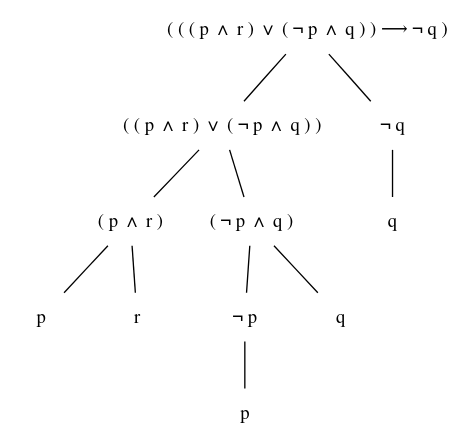
\includegraphics[scale=0.5]{c2s3ss1A.png}}
\caption{Árbol de formación de la fórmula $ (p \wedge r) \vee (\neg p \wedge q) \rightarrow \neg q$}
\end{figure}

Además LIUS posee algunas funciones que nos permiten generar estos árboles de formación para poder visualizarlos.

Utilizando la función \textit{formTree} definida en el módulo que estamos tratando, podemos generar un objeto \textit{Graph} que corresponde al árbol de formación. Para poder visualizarlo, podemos pasar dicho objeto \textit{Graph} a una \textit{String} que representa el Grafo en formato \textit{DOT}, con la función \textit{formTree2DOT}. 

\noindent\fbox{
\begin{minipage}{\textwidth - 0.3cm}
\color{gray}
\begin{center}
\underline{PROVISIONAL}
\end{center}
Para visualizarl el árbol de formación podemos utilizar una herramienta externa como \url{https://dreampuf.github.io/GraphvizOnline/}, insertando el código DOT obtenido de \textit{formTree2DOT}
\end{minipage}}

A continuación se muestra el código de implementación de las funciones anteriores. La complejidad del código reside más en aspectos técnicos relacionados con el lenguaje \textit{Elm} que en el propio algoritmo, por lo que no es necesario entender el código, es suficiente con entender el método y conocer la existencia de las funciones.\\

\newpage

\begin{lstlisting}[caption= Definición de las funciones \textit{formTree} y \textit{formTree2DOT}]
formTree : Prop -> Graph String ()
formTree x =
    case x of
        Atom psymb -> fromNodesAndEdges [Node 0 psymb] []
        Neg p -> 
            let (nodes, edges) = formTreeAux p 1 in
                fromNodesAndEdges 
                    (Node 0 (toStringProp x)::nodes) (Edge 0 1 ()::edges)
        Conj p q -> 
            let 
                (nodes1, edges1) = formTreeAux p 1
                (nodes2, edges2) = formTreeAux q 2
            in
                fromNodesAndEdges 
                    (Node 0 (toStringProp x)::(nodes1 ++ nodes2)) 
                    ([Edge 0 1 (), Edge 0 2 ()] ++ edges1 ++ edges2)

        Disj p q -> 
            let 
                (nodes1, edges1) = formTreeAux p 1
                (nodes2, edges2) = formTreeAux q 2
            in
                fromNodesAndEdges 
                    (Node 0 (toStringProp x)::(nodes1 ++ nodes2)) 
                    ([Edge 0 1 (), Edge 0 2 ()] ++ edges1 ++ edges2)
        Impl p q -> 
            let 
                (nodes1, edges1) = formTreeAux p 1
                (nodes2, edges2) = formTreeAux q 2
            in
                fromNodesAndEdges 
                    (Node 0 (toStringProp x)::(nodes1 ++ nodes2)) 
                    ([Edge 0 1 (), Edge 0 2 ()] ++ edges1 ++ edges2)
        Equi p q -> 
            let 
                (nodes1, edges1) = formTreeAux p 1
                (nodes2, edges2) = formTreeAux q 2
            in
                fromNodesAndEdges 
                    (Node 0 (toStringProp x)::(nodes1 ++ nodes2)) 
                    ([Edge 0 1 (), Edge 0 2 ()] ++ edges1 ++ edges2)
        Insat -> fromNodesAndEdges [Node 0 (toStringProp x)] []


formTreeAux : Prop -> NodeId -> (List (Node String), List (Edge ()))
formTreeAux x nodeid=
    case x of
        Atom psymb -> ([Node nodeid psymb], [])
        Neg p -> 
            let 
                nextid = Maybe.withDefault 0 
                                <| String.toInt 
                                    <| String.fromInt nodeid ++ "1" 
            in
                let 
                    (nodes, edges) = formTreeAux p nextid 
                in
                    (Node nodeid (toStringProp x)::nodes, 
                                        Edge nodeid nextid ()::edges)                               
        
        Conj p q -> 
            let 
                nextid1 =  Maybe.withDefault 0 
                                <| String.toInt 
                                    <| String.fromInt nodeid ++ "1"
                nextid2 = Maybe.withDefault 0 
                                <| String.toInt 
                                    <| String.fromInt nodeid ++ "2"
            in
                let 
                    (nodes1, edges1) = formTreeAux p nextid1
                    (nodes2, edges2) = formTreeAux q nextid2
                in
                   ( Node nodeid (toStringProp x)::(nodes1 ++ nodes2),  
                       [Edge nodeid nextid1 (), Edge nodeid nextid2 ()] ++ 
                                                           edges1 ++ edges2)
        Disj p q -> 
            let 
                nextid1 =  Maybe.withDefault 0 
                                <| String.toInt 
                                    <| String.fromInt nodeid ++ "1"
                nextid2 = Maybe.withDefault 0 
                                <| String.toInt 
                                    <| String.fromInt nodeid ++ "2"
            in
                let 
                    (nodes1, edges1) = formTreeAux p nextid1
                    (nodes2, edges2) = formTreeAux q nextid2
                in
                   ( Node nodeid (toStringProp x)::(nodes1 ++ nodes2),  
                       [Edge nodeid nextid1 (), Edge nodeid nextid2 ()] ++ 
                                                           edges1 ++ edges2)
        Impl p q -> 
            let 
                nextid1 =  Maybe.withDefault 0 
                                <| String.toInt 
                                    <| String.fromInt nodeid ++ "1"
                nextid2 = Maybe.withDefault 0 
                                <| String.toInt 
                                    <| String.fromInt nodeid ++ "2"
            in
                let 
                    (nodes1, edges1) = formTreeAux p nextid1
                    (nodes2, edges2) = formTreeAux q nextid2
                in
                   ( Node nodeid (toStringProp x)::(nodes1 ++ nodes2),  
                       [Edge nodeid nextid1 (), Edge nodeid nextid2 ()] ++ 
                                                           edges1 ++ edges2)
        
        
        
        
        
        
        
        
        
        
        
        
        
        Equi p q -> 
           let 
                nextid1 =  Maybe.withDefault 0 
                                <| String.toInt 
                                    <| String.fromInt nodeid ++ "1"
                nextid2 = Maybe.withDefault 0 
                                <| String.toInt 
                                    <| String.fromInt nodeid ++ "2"
            in
                let 
                    (nodes1, edges1) = formTreeAux p nextid1
                    (nodes2, edges2) = formTreeAux q nextid2
                in
                   ( Node nodeid (toStringProp x)::(nodes1 ++ nodes2),  
                       [Edge nodeid nextid1 (), Edge nodeid nextid2 ()] ++ 
                                                           edges1 ++ edges2)
        Insat -> ([Node nodeid (toStringProp x)], [])
        
formTree2DOT : Graph String () -> String
formTree2DOT ft =
    let myStyles =
            { defaultStyles | 
                node = "shape=plaintext, color=black"
                , edge = "dir=none"}
    in 
        outputWithStyles myStyles (\x -> Just x) (\_ -> Nothing) ft
\end{lstlisting}

\subsubsection{Principio de inducción sobre fórmulas}

Gracias a la definición de $PROP$ (y su estructura recursiva), para probar que toda fórmula proposicional satisface una cierta propiedad ($\Psi$), podemos hacerlo aplicando el método de inducción sobre fórmulas.

De esta forma, probamos:

\begin{enumerate}
\item (\textit{Caso base}). Probar que todos los elementos de $VP$ tienen la propiedad $\Psi$.
\item (\textit{Paso de inducción}).
\begin{enumerate}
\item Si $F \in PROP$ tiene la propiedad $\Psi$, entonces $\neg F$ tiene la propiedad $\Psi$.
\item Si $F, G \in PROP$, tienen la propiedad $\Psi$ entonces  $(F \wedge G), (F \vee G), (F \rightarrow G), (F \leftrightarrow G) \in PROP$ tienen la propiedad $\Psi$
\end{enumerate}
\end{enumerate}

\subsubsection{Conjuntos de fórmulas}

Definido $PROP$, los conjuntos de fórmulas no son más que subconjuntos de $PROP$, estoes, corresponden a agrupaciones de fórmulas proposicionales. 

En el lengaje LIUS, los conjuntos proposicionales se definen como listas de fórmulas proposicionales. De esta forma: \\

\begin{lstlisting}[caption= Definición de Conjunto de Fórmulas como Lista de Fórmulas Proposicionales]
type alias PropSet = List Prop
\end{lstlisting}

De forma que la definición de estos se realiza como listas de objetos \textit{Prop}. Como ejemplo, el conjunto $ \left\lbrace (p \wedge q) \vee (p \wedge r), (p \wedge r) \vee (\neg p \wedge q) \rightarrow \neg q, (p \leftrightarrow q) \wedge (p \rightarrow \neg q) \wedge p \right\rbrace$\\


\begin{lstlisting}[caption= {Ejemplo de definición de conjuntos proposicionales.}]
a : Prop
a = Disj (Conj (Atom "p") (Atom "q")) (Conj (Atom "p") (Atom "r"))
 
b : Prop   
b = Impl 
        (Disj 
            (Conj (Atom "p") (Atom "r")) 
            (Conj (Neg (Atom "p")) (Atom "q"))
        ) 
        (Neg (Atom "q"))

c : Prop
c = Conj 
        (Conj 
            (Equi (Atom "p") (Atom "q")) 
            (Impl (Atom "p") (Neg (Atom "q"))) 
        (Atom "p")

M: PropSet      
M = [a, b, c]
\end{lstlisting}

Para facilitar su escritura, en el módulo \textit{LP\_Parser}, se incluye la función \textit{parserPropSet}, que nos permite definirlos como lo hacemos con el Parser de funciones proposicionales, separando éstas por `\textit{;}'. Recomendamos vea la definición, explicación y ejemplos en el (\hyperref[sec:A1.LPParser]{\textit{\underline{Anexo A1. LP\_Parser}}}).

\subsection{Aspectos Semánticos}
\subsubsection{Interpretaciones y Valor de verdad de fórmulas proposicionales. }

Una vez provista la sintaxis, pasamos a desarrollar la semántica de la Lógica Proposicional. Como ya comentamos, hemos de abordar la interpretación de certeza o veracidad de las fórmulas. Para esto es necesario conocer los conceptos de \textit{valor de verdad} y \textit{función de verdad}.

\begin{itemize}
\item \textbf{Valor de verdad}. Los elementos del conjunto $\{0,1\}$ se denominan valores de verdad o valores booleanos. Representan si un hecho es cierto o no, de forma que el valor $1$ se asocia a \textit{verdadero} y el valor $0$ a \textit{falso}.

\item \textbf{Funciones de verdad}. Corresponden a funciones que devuelven un valor de verdad según el valor de verdad de los argumentos. Así, el significado (valor de verdad asociado) de cada una de las conectivas lógicas viene dado por una función de verdad, de forma que:

\begin{multicols}{2}
\begin{itemize}
\item 
$H_{\neg}(i) = \left\lbrace \begin{array}{l l}
1 & \textrm{si } i = 0\\
0 & \textrm{si } i = 1\\
\end{array} \right.$

\item 
$H_{\wedge}(i,j) = \left\lbrace \begin{array}{l l}
1 & \textrm{si } i = j = 1\\
0 & \textrm{e.o.c}\\
\end{array} \right.$

\item 
$H_{\vee}(i,j) = \left\lbrace \begin{array}{l l}
0 & \textrm{si } i = j = 0\\
1 & \textrm{e.o.c}\\
\end{array} \right.$

\item 
$H_{\rightarrow}(i,j) = \left\lbrace \begin{array}{l l}
0 & \textrm{si } i = 1, j = 0\\
1 & \textrm{e.o.c}\\
\end{array} \right.$

\item 
$H_{\leftrightarrow}(i,j) = \left\lbrace \begin{array}{l l}
1 & \textrm{si } i = j\\
0 & \textrm{e.o.c}\\
\end{array} \right.$
\end{itemize}
\end{multicols}

\end{itemize}

Visto esto, pasamos a estudiar el valor de verdad de las fórmulas proposicionales. Para ello debemos definir el valor de verdad de las variables proposicionales, (denominadas \textit{valoraciones} o \textit{interpretaciones}) y a partir de estas y las funciones de verdad de las conectivas,podemos extender cada valoración,$v$,de forma única,al conjunto de todas las fórmulas de manera que para cada fórmula $F$ se verifique:

\begin{multicols}{2}
\begin{itemize}
\item $v(\neg F)= H_{\neg}(v(F))$
\item $v((F \wedge G))= H_{\wedge}(v(F), v(G))$
\item $v((F \vee G))= H_{\vee}(v(F), v(G))$
\item $v((F \rightarrow G))= H_{\rightarrow}(v(F), v(G))$
\item $v((F \leftrightarrow G))= H_{\leftrightarrow}(v(F), v(G))$
\end{itemize}
\end{multicols}

Se dice que $v(F)$ es el valor de verdad de $F$ respecto de la valoración $v$.

De esta forma, es sencillo realizar el cálculo del valor de verdad de una fórmula respecto de una valoración, recurriendo al árbol de formación de la fórmula, evaluando las subfórmulas, desde las hojas (variables proposicionales) hasta el nodo raíz (la fórmula completa). Por ejemplo el cálculo de la valoración de $F \equiv \neg(\neg(p \vee q)\vee(\neg r \vee s))$ respecto de $v \equiv \{p=1, q=1, r=0, s=0\}$:

\begin{figure}[H]
\centering
\fbox{
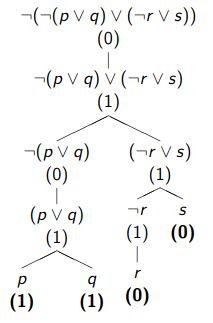
\includegraphics[scale=0.5]{c2s3ss2A.png}}
\caption{Ejmplo del cálculo de la valoración a través del árbol de formación}
\end{figure}

Para poder modelar la semántica de la LP, en el lenguaje LIUS, se han definido las estructuras necesarias que nos permitan representar las interpretaciones (o valoraciones). Para ello, hemos elegido una representación "dispersa" de manera que una interpretación corresponde a una lista de símbolos proposicionales (variables proposicionales) que son los que son considerados verdaderos, los términos que no aparecen en la lista serán considerados como falsos.\\

\begin{lstlisting}[caption= Definición de Interpretación como Lista de Símbolos Proposicionales]
type alias Interpretation = List PSymb
\end{lstlisting}

De esta forma podemos definir, de forma sencilla el valor de verdad de una fórmula respecto de una valoración. Como hemos señalado antes, el árbol de formación es equivalente a la definición recursiva que hemos adoptado para el modelado de las fórmulas proposicionales, de forma que podemos realizar el cálculo de igual forma que la presentada con el árbol de formación, de forma que:

\begin{itemize}
\item (\textit{Caso base}) Una fórmula atómica será verdadera si y sólo si el símbolo proposicional pertenece a la lista de interpretación.
\item (Casos recursivos) Según la clase de fórmula:
\begin{itemize}
\item La negación de una fórmula será verdadera respecto de una interpretación si y sólo si la evaluación de la fórmula es falsa.
\item La conjunción de dos fórmulas proposicionales será verdadera respecto de una interpretación si y sólo si la evaluación de ambas fórmulas respecto de dicha evaluación es verdadera.
\item La disyunción de dos fórmulas proposicionales será verdadera será verdadera respecto de una interpretación si y sólo si alguna de las evaluaciones de las dos fórmulas es evaluada verdadera respecto de dicha interpretación.
\item La implicación será verdadera respecto de una interpretación si y sólo si o la evaluación del antecedente es evaluado falso respecto de dicha interpretación o el consecuente es evaluado verdadero respecto de la misma.
\item La equivalencia será verdadera respecto de una interpretación si y sólo si la evaluación del antecedente coincide con la evaluación del consecuente.\\
\end{itemize} 

\begin{lstlisting}[caption= {Función de valoración de las fórmulas proposicionales}]
valuation : Prop -> Interpretation -> Bool
valuation pr i =
    case pr of
        Atom p -> List.member p i
        Neg p -> not (valuation p i)
        Conj p q -> valuation p i &&  valuation q i
        Disj p q ->   valuation p i ||  valuation q i
        Impl p q ->   not (valuation p i) ||  valuation q i
        Equi p q ->   valuation (Impl p q) i &&  valuation (Impl q p) i
\end{lstlisting}
\end{itemize}

\subsubsection{Interpretaciones. Modelos. Satisfactibilidad y Validez Lógica}

Existen métodos alternativos (pero equivalentes) para el cálculo del valor de verdad de una fórmula respecto de una valoración. Dado que, dada una valoración,$v$, el valor de verdad de una fórmula $F$ respecto de $v$ está determinado por los valores de verdad de las subfórmulas de $F$, podemos construir una tabla que recorra los valores de sus subfórmulas:

\begin{figure}[H]
\centering
\fbox{
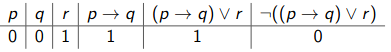
\includegraphics[scale=0.5]{c2s3ss2B.png}}
\caption{Ejmplo del cálculo de la valoración a través de tabla}
\end{figure}

Una tabla de verdad corresponde a una estructura similar a la anterior (nosotros sólo reflejaremos el valor de las variables proposicionales y el valor de verdad de la fórmula completa), en la que en cada fila se presenta la valoración y el valor de verdad de la fórmula respecto a la misma, para toda interpretación posible (que corresponda a las variables proposicionales presentes en la fórmula).

En el lenguaje LIUS, para poder construir la tabla de verdad, primero hemos de calcular todas las interpretaciones posibles, que, dada la definición dispersa que hemos adoptado, correspondería a todos los posibles subconjuntos (\textit{powerset}) que podríamos construir con los símbolos proposicionales que aparecen en la fórmula. Así:\\

\begin{lstlisting}[caption= {Función para extraer los símbolos proposicionales que intervienen en una fórmula}]
symbInProp : Prop -> Set PSymb

symbInProp f=
    case f of
        Atom p -> Set.singleton p
        Neg p -> symbInProp p
        Conj p q -> Set.union (symbInProp p ) (symbInProp q)
        Disj p q -> Set.union (symbInProp p ) (symbInProp q)
        Impl p q -> Set.union (symbInProp p ) (symbInProp q)
        Equi p q -> Set.union (symbInProp p ) (symbInProp q)
\end{lstlisting}

\begin{lstlisting}[caption= {Función para extraer las posibles interpretaciones para una fórmula propsicional}]
allInterpretations : Prop -> List Interpretation
allInterpretations x =  Aux.powerset <| List.sort <| Set.toList 
                                                         <| symbInProp x
\end{lstlisting}

De esta forma podemos expresar la tabla de verdad como una lista de tuplas en las que el primer elemento corresponde a la interpretación y el segundo corresponde a la evaluación de la fórmula respecto de dicha valoración:\\

\begin{lstlisting}[caption= {Función para la construcción de la tabla de verdad de una fórmula}]
truthTable : Prop -> List (Interpretation, Bool)
truthTable x = List.map (\xs ->  (xs,valuation x xs)) <| allInterpretations x
\end{lstlisting}

\noindent\underline{Modelos. Validez y Satisfactibilidad}

Una vez estudiado lo anterior, vamos dar unas cuantas definiciones:

\begin{itemize}
\item \textbf{Modelo.} Se dice que una fórmula $F$ es válida en una valoración $v$ o equivalentemente que $v$ es \textbf{modelo} de $F$ si $v(F)=1$ y se denota por $v \models F$. En caso contrario, se dice que $v$ es \textbf{contramodelo} de $F$ y se denota $v \not \models F$.

\item \textbf{Satisfactibilidad.} Una fórmula $F$ se dice \textbf{satisfactible} (o consistente) si existe una valoración $v$ que es modelo de $F$. En caso contrario se dice que $F$ es \textbf{insatisfactible} (o inconsistente), y se representa por $\perp$.

\item \textbf{Validez lógica o Tautología}. Una fórmula $F$ se dice \textbf{tautología} (o (lógicamente) válida) si toda valoración es modelo de $F$ y se denota $\models F$.

\end{itemize} 

\noindent \textit{Relación entre Validez y Satisfactibilidad}

\fbox{\begin{minipage}{\textwidth - 0.7cm}
LEMA: Para cada $F \in PROP$ se verifica:
\begin{enumerate}
\item Si $F$ es tautología, entonces $F$ es satisfactible.
\item $F$ es tautología si y sólo si $F$ es insatisfactible.
\end{enumerate}
\end{minipage}}

Como se ha expuesto, los modelos corresponden a las interpretaciones que son evaluadas verdaderas, esto es, de las posibles interpretaciones aquellas hacen la fórmula verdadera. Aquellas interpretaciones que hacen la fórmula falas se denominan contramodelos. Así:\\

\begin{lstlisting}[caption= {Función para el cálculo de los modelos de una fórmula proposicional}]
models : Prop -> List Interpretation
models x = List.filter (\y -> valuation x y) (allInterpretations x)

countermodels : Prop -> List Interpretation
countermodels x = List.filter (\y -> not (valuation x y)) 
                                               (allInterpretations x)
\end{lstlisting}

Definidos los modelos, podemos así mismo definir (funcionalmente) los conceptos de satisfactibilidad y validez, de acuerdo a las definiciones expuestas:\\


\begin{lstlisting}[caption={Funciones de Satisfactibilidad, Validez e Insatisfactibilidad}]
satisfactibility : Prop -> Bool
satisfactibility x = List.any (\xs-> valuation x xs) (allInterpretations x)

validity : Prop -> Bool
validity x = List.all (\xs-> valuation x xs) (allInterpretations x)

insatisfactibility : Prop -> Bool
insatisfactibility x = not (satisfactibility x)
\end{lstlisting}

\subsubsection{Conjuntos de Fórmulas. Modelos y Consistencia.}

De forma análoga a la presentada para las fórmulas proposicionales podemos definir los conceptos anteriores, aplicados a conjuntos de fórmulas de forma que:

\begin{itemize}
\item \textbf{Modelo.} Se dice que una valoración $v$ es \textbf{modelo} de un conjunto de fórmulas $U$ si para toda fórmula $F \in U$ se tiene que $v(F)=1$ y se denota por $v \models U$. En caso contrario, se dice \textbf{contramodelo}.

\item \textbf{Consistencia} Un conjunto de fórmulas $U$ se dice \textbf{consistente} si existe una valoración $v$ que es modelo de $U$. En caso contrario se dice que $U$ es \textbf{inconsistente}.
\end{itemize}

Funcionalmente la definición de los conceptos anteriores es análoga a la de las fórmulas. De forma que:\\

\begin{lstlisting}[caption={Modelos y contramodelos en conjuntos de fórmulas proposicionales}]
setSymbols : List Prop -> Set PSymb
setSymbols xs = 
    List.foldr (\x acc -> Set.union acc (symbInProp x)) Set.empty xs

allSetInterpretations : List Prop -> List Interpretation
allSetInterpretations xs = Aux.powerset <| Set.toList <| setSymbols xs
    
isSetModel : List Prop -> Interpretation -> Bool
isSetModel xs i =  List.all (\x -> valuation x i) xs

allSetModels : List Prop -> List Interpretation
allSetModels xs = List.filter (isSetModel xs) (allSetInterpretations xs)

allSetCounterModels : List Prop -> List Interpretation
allSetCounterModels xs = 
    List.filter (\x -> not(isSetModel xs x)) <| allSetInterpretations xs
\end{lstlisting}


De forma que ahora, es sencillo, comprobar la consistencia de un conjunto a partir de la definición:

\begin{lstlisting}[caption={Consistencia e Inconsistencia en Conjuntos Proposicionales}]
isConsistent : List Prop -> Bool
isConsistent xs = 
    List.any (\x -> isSetModel xs x) <| allSetInterpretations xs
    
isInconsistent: List Prop -> Bool
isInconsistent xs = not(isConsistent xs)
\end{lstlisting}

\subsubsection{Consecuencia Lógica.}

Por último nos queda definir el concepto de \textbf{consecuencia lógica}. Una fórmula $F$ es consecuencia lógica (o se sigue) de un conjunto de fórmulas $U$, y se denota por $U \models F$, si toda valoración que es modelo de $U$ es también modelo de $F$.

Es precisamente este concepto el que permite formular el problema básico en el marco de la lógica proposicional, que planteamos como objetivo de la LP.

\noindent\textit{Relación entre consecuencia lógica, consistencia y validez}

\fbox{\begin{minipage}{\textwidth - 0.7cm}
PROPOSICIÓN: Sea $\{F_1, F_2, \ldots, F_n \} \in PROP$ y $F \in PROP$ son equivalentes:
\begin{enumerate}
\item $\{F_1, F_2, \ldots, F_n \} \models F$
\item $(F_1 \wedge F_2 \wedge \ldots \wedge F_n \rightarrow F) \in TAUT$
\item $\{F_1 , F_2 , \ldots , F_n , \neg F\}\equiv \perp$
\end{enumerate}
\end{minipage}}


Funcionalmente, podemos plantear dos desarrollos alternativos para el concepto de Consecuencia Lógica:
\begin{enumerate}
\setlength{\leftskip}{0.5cm}
\item Acudiendo a la propia definición.
\item Acudiendo al tercer punto de la proposición anterior.
\end{enumerate}

\begin{lstlisting}[caption={Consecuencia Lógica}]
isConsecuence : List Prop -> Prop -> Bool
isConsecuence xs x = List.all (\y -> valuation x y) <| allSetModels xs

isConsecuence : List Prop -> Prop -> Bool
isConsecuence xs x = isInconsistent (xs ++ [Neg x])
\end{lstlisting}

\section{Algoritmos de decisión en LP}

Como hemos señalado vamos a presentar de forma somera los algoritmos de decisión en LP, e iremos desarrollando algunos de los algoritmos más importantes a lo largo de los distintos capítulos.

Dado un conjunto de fórmulas $U$, un \textbf{algoritmo de decisión} para $U$ es aquél que dada una fórmula $A \in PROP$, devuelve \texttt{SI} cuando $A \in U$ y \texttt{NO} cuando $A \not\in U$

Esto da pie a la definición de algunos problemas con un especial interés:
\begin{itemize}
\item $SAT = \{A \in PROP: \, A \textit{ es satisfactible}\}$.
\item $TAUT = \{A \in PROP: \, A \textit{ es tautología}\}$.
\item Fijado $U \subseteq PROP$, la \textbf{Teoría de $U$} corresponde a: $\mathcal{T}(U) = \{A \in PROP: \, U \models A\}$. 
\end{itemize}

Precisamente, un algoritmo de decisión para $\mathcal{T}(U)$ proporciona una respuesta al Problema Básico que planteamos al comienzo del capítulo. Por tanto, podemos reducir dicho problema a uno nuevo: Obtener un algoritmo que, dado un conjunto finito de fórmulas proposicionales, $U$, y una fórmula, $F$, decida si $U \models F$.

Y este a su vez se reduce a comprobar la satisfactibilidad de una cierta fórmula (o bien la validez de otra), hemos aquí el problema conocido como \textit{Problema $SAT$}. 

Notemos que ya hemos visto un algoritmo, el de las Tablas de Verdad, que resuelve el problema, pero la complejidad de dicho algoritmo es exponencial en el número de símbolos proposicionales, lo que lo hace inabordable para fórmulas de cierta complejidad , incluso computacionalmente.

Hemos de señalar que existen otros algoritmos de decisión del problema $SAT$, algunos de los cuales abordaremos a lo largo de los siguientes capítulos, pero aún no se ha encontrado ninguno capaz de resolver el problema eficientemente (complejidad polinomial), y, de hecho, se duda de la existencia del mismo. De hecho, determinar la satisfactibilidad de una fórmula proposicional se trata de un problema NP-completo.

\section{Origen y Conceptos Básicos de Lógica de Primer Orden}

\subsection{Limitaciones de la Lógica Proposicional}

Aunque a lógica proposicional posee un semántica sencilla y existen algoritmos de decisión (poco eficientes) para sus problemas básicos, como $SAT$ o la consecuencia lógica, la expresividad de LP es bastante limitada, esto hace que muchos problemas no sean modelables en LP, bien porque requieren un gran número de fórmulas o fórmulas de gran tamaño, o bien porque no puedan ni siquiera expresarse en este lenguaje. 
\newpage
El siguiente ejemplo presenta un razonamiento que es válido, sin embargo no es expresable en LP:
\begin{center}
1. Todo hombre es mortal. \quad 2. Sócrates es hombre. \quad 3. Por tanto, Sócrates es mortal.
\end{center}

Es aquí precisamente donde comienza el ámbito de la Lógica de Primer Orden.

\subsection{Caracterización de la Lógica de Primer Orden}

La \textbf{Lógica de Primer Orden} o \textbf{Lógica de Predicados} es un sistema formal diseñado para estudiar los métodos inferenciales en los leguajes de primer orden. Un \textbf{lenguaje de primer orden} corresponde a un lenguaje formal que consta de:

\begin{itemize}
\item \underline{Símbolos lógicos} (comunes a todos los lenguajes): En los que se engloban:
\begin{itemize}
\item Un conjunto de \textit{Variables:} $V = \{x, x_0, x_1, \ldots, y, y_0, \ldots \}$
\item \textit{Conectivas lógicas :} $\neg$ (negación), $\wedge$ (conjunción), $\vee$ (disyunción), $\rightarrow$ (implicación), $\leftrightarrow$ (equivalencia).
\item \textit{Cuantificadores:} $\exists$ (existencial), $\forall$ (universal).
\item \textit{Símbolos auxiliares:} $`('$ y $`)'$
\end{itemize}
\item \underline{Símbolos no lógicos} (propios de cada lenguaje): En los que se engloban:
\begin{itemize}
\item Un conjunto de \textit{Constantes:} $L_{C}= \{a, b, \ldots, a_{0}, a_{1}, \ldots \}$
\item Un conjunto de \textit{símbolos de función:} $L_{F} = \{f_{0}, f_{1}, \ldots\}$, cada uno con su aridad correspondiente.
\item Un conjunto de \textbf{símbolos de predicado:} $L_P=\{P_{0}, P_{1}, \ldots, Q, Q_0, \ldots\}$, cada uno con su aridad correspondiente. 

Dos notas:
\begin{itemize}
\item Los símpolos de predicado de aridad 0 actúan como símbolos proposicionales.
\item El símbolo de igualdad (`$=$') no es un predicado común a todos los lenguajes de primer orden, pero si es corriente su aparición. La familia de lenguajes que incluyen este predicado es denominada \underline{Lenguajes de Primer Orden con igualdad}.
\end{itemize}
\end{itemize}
\end{itemize}

\section{Sintáxis y Semántica en LPO Módulo SintaxSemanticLPO}
\toDo

\section{Código y funciones de los módulos presentados}
\subsection{SintaxSemanticsLP}
\subsubsection{Código del módulo}
\begin{lstlisting}[caption={Módulo SintaxSemanticsLP}, mathescape=true]
module Modules.SintaxSemanticsLP exposing (
    PSymb, Prop(..), Interpretation,PropSet,
    valuation, truthTable, models, countermodels, satisfactibility, validity, 	
    insatisfactibility, isSetModel, allSetModels, allSetCounterModels, 
    isConsistent, isInconsistent, isConsecuence, setSymbols, formTree, 
    formTree2DOT)

import List
import Set
import Modules.AuxiliarFunctions as Aux
import Graph exposing (Graph(..), Node, Edge, NodeId, fromNodesAndEdges)
import Graph.DOT exposing (outputWithStyles, defaultStyles)
import Maybe exposing (Maybe(..))

-----------
-- TYPES --
-----------
type alias PSymb = String 

type Prop = Atom PSymb
          | Neg Prop
          | Conj Prop Prop
          | Disj Prop Prop
          | Impl Prop Prop
          | Equi Prop Prop
          | Insat

type alias Interpretation = List PSymb
type alias PropSet = List Prop

-------------
-- METHODS --
-------------

formTree : Prop -> Graph String ()
formTree x =
    case x of
        Atom psymb -> fromNodesAndEdges [Node 0 psymb] []
        Neg p -> 
            let (nodes, edges) = formTreeAux p 1 in
                fromNodesAndEdges 
                    (Node 0 (toStringProp x)::nodes) (Edge 0 1 ()::edges)
        Conj p q -> 
            let 
                (nodes1, edges1) = formTreeAux p 1
                (nodes2, edges2) = formTreeAux q 2
            in
                fromNodesAndEdges 
                    (Node 0 (toStringProp x)::(nodes1 ++ nodes2)) 
                    ([Edge 0 1 (), Edge 0 2 ()] ++ edges1 ++ edges2)

        Disj p q -> 
            let 
                (nodes1, edges1) = formTreeAux p 1
                (nodes2, edges2) = formTreeAux q 2
            in
                fromNodesAndEdges 
                    (Node 0 (toStringProp x)::(nodes1 ++ nodes2)) 
                    ([Edge 0 1 (), Edge 0 2 ()] ++ edges1 ++ edges2)
        Impl p q -> 
            let 
                (nodes1, edges1) = formTreeAux p 1
                (nodes2, edges2) = formTreeAux q 2
            in
                fromNodesAndEdges 
                    (Node 0 (toStringProp x)::(nodes1 ++ nodes2)) 
                    ([Edge 0 1 (), Edge 0 2 ()] ++ edges1 ++ edges2)
        Equi p q -> 
            let 
                (nodes1, edges1) = formTreeAux p 1
                (nodes2, edges2) = formTreeAux q 2
            in
                fromNodesAndEdges 
                    (Node 0 (toStringProp x)::(nodes1 ++ nodes2)) 
                    ([Edge 0 1 (), Edge 0 2 ()] ++ edges1 ++ edges2)
        Insat -> fromNodesAndEdges [Node 0 (toStringProp x)] []


formTreeAux : Prop -> NodeId -> (List (Node String), List (Edge ()))
formTreeAux x nodeid=
    case x of
        Atom psymb -> ([Node nodeid psymb], [])
        Neg p -> 
            let 
                nextid = Maybe.withDefault 0 
                                <| String.toInt 
                                    <| String.fromInt nodeid ++ "1" 
            in
                let 
                    (nodes, edges) = formTreeAux p nextid 
                in
                    (Node nodeid (toStringProp x)::nodes, 
                                        Edge nodeid nextid ()::edges)                               
        
        Conj p q -> 
            let 
                nextid1 =  Maybe.withDefault 0 
                                <| String.toInt 
                                    <| String.fromInt nodeid ++ "1"
                nextid2 = Maybe.withDefault 0 
                                <| String.toInt 
                                    <| String.fromInt nodeid ++ "2"
            in
                let 
                    (nodes1, edges1) = formTreeAux p nextid1
                    (nodes2, edges2) = formTreeAux q nextid2
                in
                   ( Node nodeid (toStringProp x)::(nodes1 ++ nodes2),  
                       [Edge nodeid nextid1 (), Edge nodeid nextid2 ()] ++ 
                                                           edges1 ++ edges2)
        Disj p q -> 
            let 
                nextid1 =  Maybe.withDefault 0 
                                <| String.toInt 
                                    <| String.fromInt nodeid ++ "1"
                nextid2 = Maybe.withDefault 0 
                                <| String.toInt 
                                    <| String.fromInt nodeid ++ "2"
            in
                let 
                    (nodes1, edges1) = formTreeAux p nextid1
                    (nodes2, edges2) = formTreeAux q nextid2
                in
                   ( Node nodeid (toStringProp x)::(nodes1 ++ nodes2),  
                       [Edge nodeid nextid1 (), Edge nodeid nextid2 ()] ++ 
                                                           edges1 ++ edges2)
        Impl p q -> 
            let 
                nextid1 =  Maybe.withDefault 0 
                                <| String.toInt 
                                    <| String.fromInt nodeid ++ "1"
                nextid2 = Maybe.withDefault 0 
                                <| String.toInt 
                                    <| String.fromInt nodeid ++ "2"
            in
                let 
                    (nodes1, edges1) = formTreeAux p nextid1
                    (nodes2, edges2) = formTreeAux q nextid2
                in
                   ( Node nodeid (toStringProp x)::(nodes1 ++ nodes2),  
                       [Edge nodeid nextid1 (), Edge nodeid nextid2 ()] ++ 
                                                           edges1 ++ edges2)

        Equi p q -> 
           let 
                nextid1 =  Maybe.withDefault 0 
                                <| String.toInt 
                                    <| String.fromInt nodeid ++ "1"
                nextid2 = Maybe.withDefault 0 
                                <| String.toInt 
                                    <| String.fromInt nodeid ++ "2"
            in
                let 
                    (nodes1, edges1) = formTreeAux p nextid1
                    (nodes2, edges2) = formTreeAux q nextid2
                in
                   ( Node nodeid (toStringProp x)::(nodes1 ++ nodes2),  
                       [Edge nodeid nextid1 (), Edge nodeid nextid2 ()] ++ 
                                                           edges1 ++ edges2)
        Insat -> ([Node nodeid (toStringProp x)], [])
        
formTree2DOT : Graph String () -> String
formTree2DOT ft =
    let myStyles =
            { defaultStyles | 
                node = "shape=plaintext, color=black"
                , edge = "dir=none"}
    in 
        outputWithStyles myStyles (\x -> Just x) (\_ -> Nothing) ft


valuation : Prop -> Interpretation -> Bool
valuation pr i =
    case pr of
        Atom p -> List.member p i
        Neg p -> not (valuation p i)
        Conj p q -> valuation p i &&  valuation q i
        Disj p q ->   valuation p i ||  valuation q i
        Impl p q ->   not (valuation p i) ||  valuation q i
        Equi p q ->   valuation (Impl p q) i &&  valuation (Impl q p) i
        Insat -> Basics.False

symbInProp : Prop -> Set.Set PSymb

symbInProp f=
    case f of
        Atom p -> Set.singleton p
        Neg p -> symbInProp p
        Conj p q -> Set.union (symbInProp p ) (symbInProp q)
        Disj p q -> Set.union (symbInProp p ) (symbInProp q)
        Impl p q -> Set.union (symbInProp p ) (symbInProp q)
        Equi p q -> Set.union (symbInProp p ) (symbInProp q)
        Insat -> Set.empty

allInterpretations : Prop -> List Interpretation
allInterpretations x =  Aux.powerset <| List.sort <| Set.toList 
                                                      <| symbInProp x

truthTable : Prop -> List (Interpretation, Bool)
truthTable x = List.map (\xs ->  (xs,valuation x xs)) <| allInterpretations x

models : Prop -> List Interpretation
models x = List.filter (\y -> valuation x y) (allInterpretations x)

countermodels : Prop -> List Interpretation
countermodels x = List.filter (\y -> not(valuation x y)) 
                              (allInterpretations x)

satisfactibility : Prop -> Bool
satisfactibility x = List.any (\xs-> valuation x xs) (allInterpretations x)

validity : Prop -> Bool
validity x = models x== allInterpretations x

insatisfactibility : Prop -> Bool
insatisfactibility x = List.isEmpty (models x)

setSymbols : List Prop -> Set.Set PSymb
setSymbols xs = List.foldr (\x acc -> Set.union acc (symbInProp x)) 
                           Set.empty 
                           xs

allSetInterpretations : List Prop -> List Interpretation
allSetInterpretations xs = Aux.powerset <| Set.toList <| setSymbols xs

isSetModel : List Prop -> Interpretation -> Bool
isSetModel xs i =  List.all (\x -> valuation x i) xs

allSetModels : List Prop -> List Interpretation
allSetModels xs = List.filter (isSetModel xs) (allSetInterpretations xs)

allSetCounterModels : List Prop -> List Interpretation
allSetCounterModels xs = List.filter (\x -> not(isSetModel xs x)) 
                                     (allSetInterpretations xs)

isConsistent : List Prop -> Bool
isConsistent xs = List.any (\x -> isSetModel xs x)
                           (allSetInterpretations xs)

isInconsistent: List Prop -> Bool
isInconsistent xs = not(isConsistent xs)

isConsecuence : List Prop -> Prop -> Bool
--isConsecuence xs x = List.all (\y -> valuation x y) <| allSetModels xs
isConsecuence xs x = isInconsistent (xs ++ [Neg x])
\end{lstlisting}

\subsubsection{Funciones disponibles}

\begin{table}[H]
\centering
\begin{tabular}{p{3cm} p{13.2cm}}
\hline
Tipo & Descripción\\
\hline
\hline
\textit{PSymb} & Alias de \textit{String}. Representa los símbolos proposicionales.\\
\hline
\textit{Prop}& Representa a las proposiciones o fórmulas proposicionales. Posee varios constructores según el tipo de fórmula proposicional: (\textit{Atom, Neg, Conj, Disj, Impl, Equi}).\\
\hline
\textit{Interpretation}& Alias de \textit{List PSymb}. Representa una interpretación, de forma que se consideran verdaderos los símbolos proposicionales que aparecen en la lista, y falsos aquellos que no aparecen.\\
\hline
\textit{PropSet}& Alias de \textit{List Prop}. Representa conjuntos de fórmulas.\\
\hline
\end{tabular}
\caption{Módulo SintaxSemanticsLP I. Tipos}
\vspace{0.5cm}
\begin{tabular}{p{3cm} p{13.2cm}}
\hline
Método & Descripción\\
\hline
\hline
\textit{formTree}& \textit{formTree: Prop -> Graph String ()}\\
& Genera un grafo con el árbol de formación de la fórmula dada.\\
\hline
\textit{formTree2DOT}& \textit{formTree2DOT: Graph String () -> String}\\
& Genera el una cadena con el código en formato DOT del árbol de formación recibido.\\
\hline
\textit{valuation}& \textit{valuation: Prop -> Interpretation -> Prop}\\
& Calcula el valor de verdad de una proposición según la interpretación dada.\\
\hline
\textit{truthTable}& \textit{truthTable: Prop -> List (Interpretation, Bool
)}\\
& Calcula la tabla de verdad asociada a una fórmula proposicional, devolviéndola como una lista de pares (Interpretación, Valoración).\\
\hline
\textit{models}& \textit{models: Prop -> List Interpretation}\\
& Calcula los modelos de una fórmula proposicional.\\
\hline
\textit{countermodels}& \textit{countermodels: Prop -> List Interpretation}\\
& Calcula los contramodelos de una fórmula proposicional.\\
\hline
\textit{satisfactibility}& \textit{satisfactibility: Prop -> Bool}\\
& Decide si una fórmula proposicional es satisfactible o no.\\
\hline
\textit{validity}& \textit{validity: Prop -> Bool}\\
& Decide si una fórmula proposicional es tautología o no.\\
\hline
\textit{insatisfactibility}& \textit{insatisfactibility: Prop -> Bool}\\
& Decide si una fórmula proposicional es insatisfactible o no.\\
\hline
\textit{isSetModel}& \textit{isSetModel: List Prop -> Interpretation ->Bool}\\
& Decide si una interpretación es modelo de un conjunto de fórmulas proposicionales o no.\\
\hline
\textit{allSetModels}& \textit{allSetModels: List Prop -> List Interpretation}\\
& Calcula los modelos asociados a un conjunto de fórmulas proposicionales.\\
\hline
\textit{allSetCounterModels}& \textit{allSetCounterModels: List Prop -> List Interpretation}\\
& Calcula los contramodelos asociados a un conjunto de fórmulas proposicionales.\\
\hline
\textit{isConsistent}& \textit{isConsistent: List Prop -> Bool}\\
& Decide si un conjunto de fórmulas proposicionales es consistente o no.\\
\hline
\textit{isInconsistent}& \textit{isInconsistent: List Prop -> Bool}\\
& Decide si un conjunto de fórmulas proposicionales es inconsistente o no.\\
\hline
\textit{isConsecuence}& \textit{isConsecuence: List Prop -> Prop -> Bool}\\
& Decide si una fórmula es consecuencia lógica de un conjunto de fórmulas proposicionales.\\
\hline
\end{tabular}
\caption{Módulo SintaxSemanticsLP II. Funciones}
\end{table}

\newpage
\subsection{SintaxSemanticsLPO}
\toDo

\section{Ejercicios Propuestos}
\toDo

\section{Resolución de los ejercicios propuestos utilizando LIUS}
\label{sec:2.7}

\toDo

\appendix
\clearpage
\addappheadtotoc
\appendixpage
\chapter{Parsers}
\newpage
\section{Módulo LP\_Parser}
\label{sec:A1.LPParser}

\toDo

\end{document}
